\section{Мета практикуму}

Ознайомлення з пiдходами побудови атак на асиметричнi криптосистеми на прикладi атак на криптосистему RSA, а саме атаки на основi китайської теореми про лишки, що є успiшною при використаннi однакового малого  значення вiдкритої експоненти для багатьох користувачiв, та атаки <<зустрiч посерединi>>, яка можлива у випадку, якщо шифротекст є невеликим числом, що є добутком двох чисел.

Практично ознайомитися із принципами статистичних методiв розрiзнення змiстовного тексту вiд випадкової послiдовностi, порівняти їх.

\subsection{Постановка задачі та варіант}
У даній роботі виконував варіант №4 як і звичайний так і простий длля атаки малої експоненти, а для атаки посередині використовую простий варіант та простіший так як у бібліотеці погано працює піднесення до степеня. Усі файли, що були використані для обчислень наведені на гіт репозиторії.


\begin{tabularx}{\textwidth}{X|X}
	\textbf{Треба виконати} & \textbf{Зроблено} \\
	Провести атаки та навести результати включно із часом їх виконання & \checkmark \\
\end{tabularx}


\section{Хід роботи/Опис труднощів}
    У ході роботи над даною лабораторною роботою було дуже просто реалізовано атаку малої експоненти, так як код для вирішення ситеми рівнянь уже був готовий і реалізований у попередніх лабах із асиметричної криптографії. Якщо говорити щодо атаки <<зустріч посередині>>, то чомусь думав, що код не працює, а це лише довго обчислювалося піднесення до степеня. Якщо не враховувати свої власні непопрозуміння, то проблем особливих не було.

\section{Результати дослідження}
У ході роботи було успішно на практиці проведено атаку на основі Китайської теореми про лишки та атаку <<зустріч посередині>>.

\section{Результат проведення атаки на основі Китайської теореми про лишки}
Атака була проведено успішно, адже значення ШТ та $m^e$ співпали.

        \begin{figure}[!h]
            \centering
            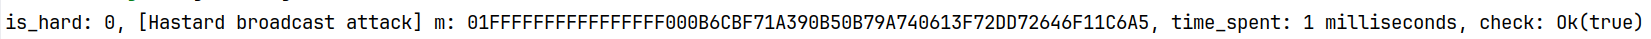
\includegraphics[scale=0.3]{Images/chinese_easy.png}
            \caption{Атака на легкий варіант.}
            \label{fig:chinese_easy}
        \end{figure}

        \begin{figure}[!h]
            \centering
            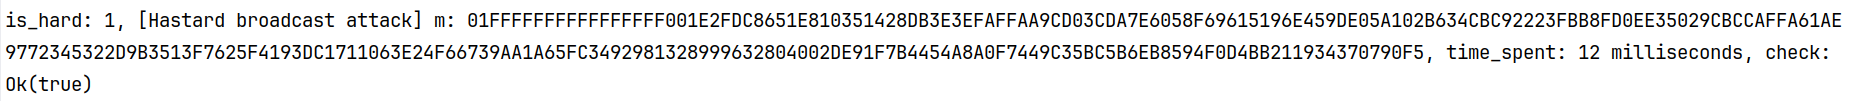
\includegraphics[scale=0.25]{Images/chinese_normal.png}
            \caption{Атака на звичайний варіант.}
            \label{fig:chinese_hard}
        \end{figure}

В результаті проведедння атаки отримав такі часові результати:
\begin{itemize}
    \item для легкого варіанту \textbf{time.spent} $=0.001804$ секунди;  
    \item для звичайного варіанту \textbf{time.spent} $=0.0514$ секунди.
\end{itemize}

\section{Результат проведення атаки <<зустріч посередині>>}
Атака була проведено успішно, адже значення ШТ та $m^e$ співпали.

\begin{figure}[!h]
            \centering
            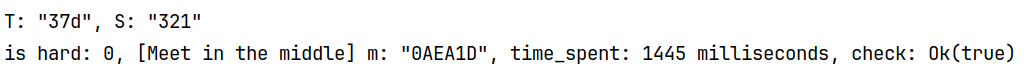
\includegraphics[scale=0.4]{Images/meet_in_middle_easy.png}
            \caption{Атака на легкий варіант разом із повідомленням m та перевіркою на правильність.}
            \label{fig:middle_easy}
        \end{figure}

\begin{figure}[!h]
            \centering
            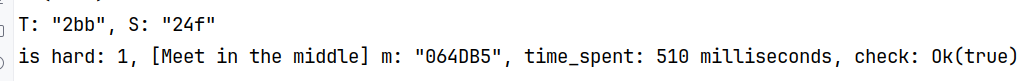
\includegraphics[scale=0.4]{Images/meet_in_middle_easiest.png}
            \caption{Атака на найлегший варіант разом із повідомленням m та перевіркою на правильність.}
            \label{fig:middle_easy}
        \end{figure}


В результаті проведедння атаки отримав такі часові результати:
\begin{itemize}
    \item для найлегшого варіанту \textbf{time.spent} $=0.51$ секунд; 
    \item для легкого варіанту \textbf{time.spent} $=1.445$ секунд;  
    \item для звичайного варіанту \textbf{time.spent} $=?$ не зміг дочекатися.
\end{itemize}

\subsection{Маленьке порівняння швидкодії із повним перебором}
На жаль, не проводилося, так як бачу скільки програма виконувала звичайний варіант по часу, не думаю, що саме моя програма виконає перебір швидше, буде тільки довше.

\section{Висновки}
В даному практикумі за допомогою програмної реалізації на практиці ознайомилися із пiдходами побудови атак на асиметричнi криптосистеми на прикладi атак на криптосистему RSA, а саме атаки на основi китайської теореми про лишки та атаки <<зустрiч посерединi>>. Перша атака вийшла добре, але друга за допомоги неоптимізованої реалізації працює дуже довго. Щоб покащити алгортими досить будде використати інший крейт із ефективнішою операцією піднесення до степеня.
% \begin{figure}
%     \centering
%     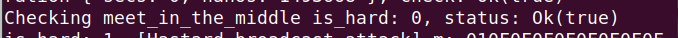
\includegraphics[width=0.5\linewidth]{middle_easy_check.png}
%     \caption{Enter Caption}
%     \label{fig:enter-label}
% \end{figure}
